\section{Adapter-Muster}

\subsection{Problemstellung}
Man m"ochte ein "ahnliches Objekt in gleicher Weise verarbeiten. Wie man es mit einer geg. Objektinstanz tun w"urde. 

\paragraph{Beispiel aus dem Buch}
Man m"ochte eine Truthahn-Instanz in gleicher Weise wie eine Enten-Instanz verwalten. Beide sind in der Lage Laute von sich zu geben und (zumindest kurze Strecken) zu fliegen. Ein Adapter-Interface erm"oglicht dies. Der Klient arbeitet nun mit diesem Adapter welcher von dem Enten-Interface erbt. Das Interface tut nun nichts anderes als entsprechenden Methoden einer Instanzvariablen aufzurufen, er dient in gewisser Weise als "Ubersetzer. 

\subsection{Erkl"arung des Musters}
Das Adapter Muster konvertiert ein geg. Interface einer Klasse in eins welches vom Klienten erwartet wird. Adapter lassen verschiedene Klassen zusammenarbeiten welche dies sonst nicht ohne weiteres k"onnten. 

\begin{figure}[b!]
	\centering
	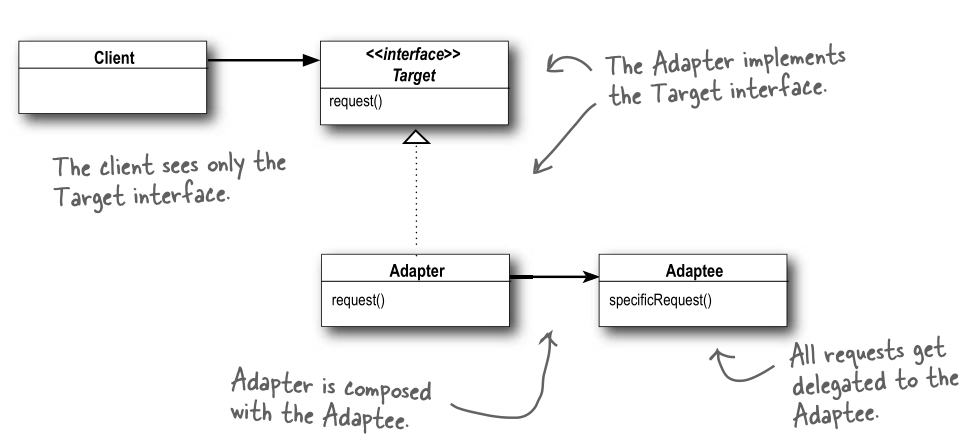
\includegraphics[width=1\linewidth]{adapter/img/adapterUML}
	\caption{UML-Darstellung des Adapter-Musters}
	\label{fig:adapterUML}
\end{figure}

\subsection{Sonderfall: Facade-Muster}
\paragraph{Problemstellung}
Klient besitzt neues Heimkino. Alle Projektoren, Hifi und sonstige Anlagen jedes Mal \emph{per Hand} zu starten / beenden ist nervig. Das Facade-Muster versteckt diese low-level Zugriffe hinter einem Interface. 

Vorteile: Teilweises Entkoppeln des Klients von Low-level-Komponenten (falls gew"unscht besitzt der Klient weiterhin Zugriff auf die Komponenten). Vereinfacht die Nutzung der Komponenten stark und es ist sogar m"oglich mehrere verschiedene Interfaces f"ur verschiedene Anwendungszwecke zu bauen (hohe Flexibilit"at). 
